% Figure: F02 in full. A multi-scale EfficientNetV2-S under a 2-layer
% transformer. F01 is the same encoder under GRU-128.
% Build: pdflatex fig_f02.tex
\documentclass[border=2pt]{standalone}
% One look for every architecture figure. Change a colour or font here, once.
\PassOptionsToPackage{table}{xcolor}
\usepackage[T1]{fontenc}
\usepackage{lmodern}
\renewcommand{\familydefault}{\sfdefault}
\usepackage{amsmath}
\usepackage{array}
\usepackage{graphicx}
\usepackage{fontawesome5}
\usepackage{tikz}
\usetikzlibrary{positioning, arrows.meta, fit, backgrounds, calc,
  decorations.pathreplacing}

% colour says where the weights came from, nothing else
\definecolor{preEdge}{RGB}{0,94,150}      % pretrained weights
\definecolor{preFill}{RGB}{214,232,245}
\definecolor{newEdge}{RGB}{176,92,0}      % new weights, trained from scratch
\definecolor{newFill}{RGB}{253,229,196}
\definecolor{opEdge}{RGB}{120,120,120}    % no weights
\definecolor{opFill}{RGB}{236,236,236}
\definecolor{ink}{RGB}{35,35,35}
\definecolor{note}{RGB}{90,90,90}
\definecolor{groupFill}{RGB}{245,245,245}
\definecolor{stripe}{RGB}{243,243,243}
% boxes drawn on photos: Okabe-Ito, readable on grass
\definecolor{strikerBox}{RGB}{0,114,178}
\definecolor{batBox}{RGB}{204,121,167}
\definecolor{cropBox}{RGB}{230,159,0}

% the icon says whether the weights move during training
\newcommand{\frozen}{{\color{ink}\faSnowflake[regular]}}
\newcommand{\trained}{{\color{ink}\faFire}}

% a small filled square for legends; no tikz inside tikz
\newcommand{\swatch}[2]{{\setlength{\fboxsep}{0pt}\setlength{\fboxrule}{0.6pt}%
  \fcolorbox{#1}{#2}{\rule{0pt}{1.4ex}\rule{2.2ex}{0pt}}}}
\newcommand{\archlegend}{\swatch{preEdge}{preFill}~pretrained weights\quad
  \swatch{newEdge}{newFill}~new weights\quad
  \swatch{opEdge}{white}~no weights\qquad
  \frozen~frozen\quad \trained~trained}

% tensor sizes
\newcommand{\by}{\ensuremath{\times}}
\newcommand{\sq}{\textsuperscript{2}}
\newcommand{\dims}[1]{#1}
\newcommand{\arrowto}{\ensuremath{\to}}

\tikzset{
  every node/.style={font=\footnotesize, text=ink},
  flow/.style={-{Stealth[length=2.2mm, width=1.7mm]}, line width=0.75pt,
    draw=ink},
  box/.style={rounded corners=2pt, line width=0.7pt, align=center,
    minimum height=8mm, inner sep=3pt,
    execute at begin node={\hyphenpenalty=10000\exhyphenpenalty=10000}},
  pre/.style={box, draw=preEdge, fill=preFill},
  new/.style={box, draw=newEdge, fill=newFill},
  op/.style={box, draw=opEdge, fill=white},
  group/.style={rounded corners=3pt, draw=opEdge, dashed, line width=0.5pt,
    fill=groupFill, inner sep=4pt},
  grouplabel/.style={font=\scriptsize, text=note, inner sep=1pt},
  % a tensor size, sitting on its arrow so it never crosses a line
  dim/.style={font=\scriptsize, text=ink, fill=white, draw=opEdge!55,
    line width=0.3pt, rounded corners=1.5pt, inner sep=1.1pt},
  size/.style={font=\scriptsize, text=note, inner sep=1.5pt,
    execute at begin node={\hyphenpenalty=10000\exhyphenpenalty=10000}},
  tag/.style={font=\scriptsize\bfseries, inner sep=1pt},
  legend/.style={font=\scriptsize, text=note, inner sep=2pt},
  frame/.style={inner sep=0pt, draw=ink!55, line width=0.3pt},
  letter/.style={font=\footnotesize\bfseries, inner sep=0pt},
  % a box opening up into the table that lists its options
  cone/.style={fill=#1, fill opacity=0.45, draw=none},
  conelink/.style={draw=opEdge!80, line width=0.4pt, densely dashed},
  bone/.style={line width=1.0pt, draw=white, line cap=round},
  guess/.style={line width=0.8pt, draw=white, dash pattern=on 1.6pt off 1.2pt},
  joint/.style={fill=cropBox},
  guessjoint/.style={fill=white},
}

% a clip as a deck of three of its frames; #1 name, #2 where, #3 width
\newcommand{\clipdeck}[3]{%
  \node[frame] (#1-c) at ($(#2)+(0.22,0.22)$)
    {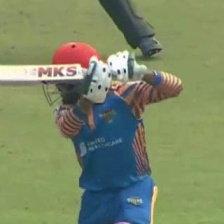
\includegraphics[width=#3]{img/crop15.jpg}};
  \node[frame] (#1-b) at ($(#2)+(0.11,0.11)$)
    {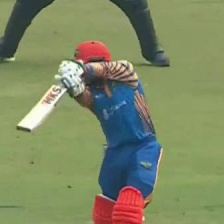
\includegraphics[width=#3]{img/crop08.jpg}};
  \node[frame] (#1-a) at (#2) {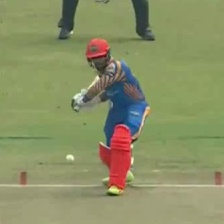
\includegraphics[width=#3]{img/crop01.jpg}};
  \node[fit=(#1-a)(#1-b)(#1-c), inner sep=0pt] (#1) {};
}

% a table card: a header band in the colour of the box it opens up.
% #1 name, #2 top-left corner, #3 band fill, #4 edge, #5 title, #6 a tabular
\newcommand{\card}[6]{%
  \node[anchor=north west, inner sep=0pt, fill=white, font=\scriptsize]
    (#1) at ([yshift=-5mm]#2) {#6};
  \node[fit={(#1.north west)([yshift=5mm]#1.north east)}, inner sep=0pt,
    fill=#3] (#1-head) {};
  \node[anchor=west, inner sep=0pt, font=\footnotesize\bfseries]
    at ([xshift=4pt]#1-head.west) {#5};
  \draw[#4, line width=0.7pt] (#1-head.north west) rectangle (#1.south east);
  \draw[#4, line width=0.5pt] (#1-head.south west) -- (#1-head.south east);
}
% rows inside a card
\newcommand{\cardrule}{\arrayrulecolor{opEdge!60}\hline}
\newcommand{\grouprow}[2]{\rowcolor{white}%
  \multicolumn{#1}{l}{\rule{0pt}{2.6ex}\textbf{\color{note}#2}}\\}
\newcolumntype{P}[1]{>{\raggedright\arraybackslash}p{#1}}
\newcommand{\cardtable}[2]{{\setlength{\tabcolsep}{4pt}%
  \hyphenpenalty=10000\exhyphenpenalty=10000%
  \renewcommand{\arraystretch}{1.12}\rowcolors{2}{white}{stripe}%
  \begin{tabular}{#1}#2\end{tabular}}}
% the shaded zoom from a box (#1) down to its card (#2), colour #3
\newcommand{\zoomto}[3]{%
  \begin{scope}[on background layer]
    \fill[cone=#3] (#1.south west) -- (#1.south east) --
      (#2-head.north east) -- (#2-head.north west) -- cycle;
  \end{scope}
  \draw[conelink] (#1.south west) -- (#2-head.north west);
  \draw[conelink] (#1.south east) -- (#2-head.north east);
}


\begin{document}
\begin{tikzpicture}[
  stage/.style={pre, text width=1.3cm, font=\scriptsize, inner sep=2pt},
  tap/.style={op, text width=1.95cm, font=\scriptsize, inner sep=2pt,
    minimum height=7mm},
  layer/.style={new, font=\scriptsize, inner sep=2pt, minimum height=7mm},
  sum/.style={circle, draw=opEdge, fill=white, line width=0.7pt,
    inner sep=0pt, minimum size=4.6mm, font=\footnotesize},
  zoom/.style={draw=opEdge, line width=0.4pt, densely dashed}]

% ---- the encoder, one frame ----
\node[frame, anchor=west] (img) at (0,0)
  {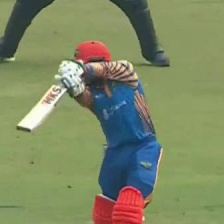
\includegraphics[width=1.45cm]{img/crop08.jpg}};
\node[size, anchor=north, align=center] at (img.south)
  {one frame\\3\by224\textsuperscript{2}};

\node[stage, minimum height=1.25cm, right=0.75cm of img] (s13) {Stem and\\stages 1--3};
\node[stage, minimum height=0.95cm, right=1.35cm of s13] (s45) {Stages 4--5};
\node[stage, minimum height=0.75cm, right=1.35cm of s45] (s67) {Stages 6--7};
\draw[flow] (img) -- (s13);
\draw[flow] (s13) -- node[size, above] {64\by28\textsuperscript{2}} coordinate[pos=0.42] (t3) (s45);
\draw[flow] (s45) -- node[size, above] {160\by14\textsuperscript{2}} coordinate[pos=0.42] (t5) (s67);

% the two inner maps, normalised and shrunk to the last grid
\node[tap, anchor=north] (tapA) at ([yshift=-0.95cm]t3) {BatchNorm, no scale;\\pool to 7\by7};
\node[tap, anchor=north] (tapB) at ([yshift=-0.95cm]t5) {BatchNorm, no scale;\\pool to 7\by7};
\node[op, font=\scriptsize, minimum height=7mm, inner sep=2pt, text width=1.15cm,
  anchor=center] (cat) at ([xshift=1.35cm]s67.east |- tapB.center) {concat\\channels};
\node[op, font=\scriptsize, minimum height=7mm, inner sep=2pt, right=1.25cm of cat] (flat) {flatten};
\fill[ink] (t3) circle (1.1pt);
\fill[ink] (t5) circle (1.1pt);
\draw[flow] (t3) -- (tapA);
\draw[flow] (t5) -- (tapB);
\draw[flow] (tapB) -- node[size, above] {160\by7\textsuperscript{2}} (cat);
\coordinate (dip) at ([yshift=-0.4cm]tapA.south);
\draw[flow] (tapA.south) -- (dip) -| node[size, below, pos=0.25] {64\by7\textsuperscript{2}} (cat.south);
\draw[flow] (s67.east) -| node[size, above, pos=0.3] {1,280\by7\textsuperscript{2}} (cat.north);
\draw[flow] (cat) -- node[size, above] {1,504\by7\textsuperscript{2}} (flat);

\begin{scope}[on background layer]
  \node[group, fit=(img)(s13)(s67)(tapA)(cat)(flat)(dip), inner sep=6pt,
    inner ysep=9pt] (enc) {};
\end{scope}
\node[grouplabel, anchor=south] at (enc.north)
  {EfficientNetV2-S, ImageNet, fine-tuned: 20.2 M weights, shared by all 15 frames};

% ---- the head, all 15 frames ----
\node[layer, text width=1.9cm, anchor=north west] (proj)
  at ([yshift=-1.0cm]enc.south west)
  {\textbf{Linear}\\73,696\,\arrowto\,256\\{\color{note}18.9 M weights}};
\node[sum, right=0.95cm of proj] (addpos) {$+$};
\node[layer, text width=1.75cm, below=0.4cm of addpos] (pos)
  {a learned position for each frame};
\node[layer, text width=2.1cm, minimum height=1.2cm, right=0.6cm of addpos] (encl)
  {\textbf{\footnotesize Transformer\\encoder layer}\\pre-norm, 4 heads};
\node[font=\footnotesize\bfseries, anchor=west, inner sep=1pt] (x2) at (encl.east) {\,\by2};
\node[op, font=\scriptsize, text width=1.4cm, minimum height=7mm, inner sep=2pt,
  right=1.05cm of x2] (mean) {mean over\\the 15 frames};
\node[layer, text width=1.95cm, right=0.6cm of mean] (cls)
  {\textbf{Classifier}\\BatchNorm\\FC 1,024, ReLU\\FC 15};
\node[right=0.45cm of cls, align=center, inner sep=1pt] (out) {\textbf{Cover}\\\textbf{Drive}};

\draw[flow] (flat.south) |- node[size, above, pos=0.75] {15\by73,696 (the 15 frames, in order)}
  ([yshift=5mm]proj.north) -- (proj.north);
\draw[flow] (proj) -- node[size, above] {15\by256} (addpos);
\draw[flow] (pos) -- (addpos);
\draw[flow] (addpos) -- (encl);
\draw[flow] (x2) -- node[size, above] {15\by256} (mean);
\draw[flow] (mean) -- node[size, above] {256} (cls);
\draw[flow] (cls) -- (out);

% ---- one encoder layer, enlarged ----
\node[layer, anchor=north west, text width=1.22cm] (ln1)
  at ([xshift=0.75cm, yshift=-1.6cm]encl.south west) {LayerNorm};
\node[layer, right=0.38cm of ln1, text width=1.55cm] (mhsa) {self-attention\\4 heads};
\node[sum, right=0.38cm of mhsa] (r1) {$+$};
\node[layer, right=0.5cm of r1, text width=1.22cm] (ln2) {LayerNorm};
\node[layer, right=0.38cm of ln2, text width=1.95cm] (ffn) {feed-forward\\256\,\arrowto\,512\,\arrowto\,256};
\node[sum, right=0.38cm of ffn] (r2) {$+$};
\coordinate (inA) at ([xshift=-0.5cm]ln1.west);
\coordinate (outA) at ([xshift=0.4cm]r2.east);
\draw[flow] (inA) -- (ln1);
\draw[flow] (ln1) -- (mhsa);
\draw[flow] (mhsa) -- (r1);
\draw[flow] (r1) -- (ln2);
\draw[flow] (ln2) -- (ffn);
\draw[flow] (ffn) -- (r2);
\draw[flow] (r2) -- (outA);
\draw[flow] ([xshift=0.2cm]inA) -- ++(0,0.6) -| (r1.north);
\draw[flow] ([xshift=0.27cm]r1.east) -- ++(0,0.6) -| (r2.north);
\begin{scope}[on background layer]
  \node[group, fit=(inA)(ln1)(r2)(outA), inner sep=4pt, inner ysep=10pt,
    yshift=3pt] (zoombox) {};
\end{scope}
\node[grouplabel, anchor=north] at (zoombox.south)
  {one encoder layer, enlarged; ReLU, no dropout};
\draw[zoom] (encl.south west) -- (zoombox.north west);
\draw[zoom] (encl.south east) -- (zoombox.north east);

% ---- legend ----
\node[legend, anchor=north, align=center] at ($(current bounding box.south)+(0,-1.5mm)$)
  {\swatch{preEdge}{preFill}~pretrained weights, fine-tuned\quad
   \swatch{newEdge}{newFill}~new weights, trained\quad
   \swatch{opEdge}{white}~no weights\\
   F01 is the same encoder under GRU-128 and the same classifier};
\end{tikzpicture}
\end{document}
